\chapter{Adding Memory to the Agents}
\section{Overview}
In the previous chapters, we have assumed that the agents interact in fully observable problems, following an MDP. This means that the observation that the agent receives from the environment is sufficient to fully understand its state. Thus:

\begin{equation}
    o_{t} = s_{t}
\end{equation}

But this is not always true. In robotics problems, robots observe its environment through sensors, and, commonly, the data obtained from them gives partial information about the robot's state. So, a significant set of real-world problems is better described by POMDPs.

There are different reason of why a problem could be partially observed. One of them is when a state is described by time-dependent phenomena, and the observations only get partial information about them. For instance, an agent could need to estimate the velocity of a flying drone by getting instant RGB snapshots of its movements. Unless observations from different time steps are combined, the agent is not going to be able to make this estimation. Other examples of time-dependent phenomena that do not have to do with the dynamics of the environment are temporary occlusions or corrupted communication systems between the sensors and the agent. From now on, we are going to use the acronym POMDP to refer to the just mentioned set of POMDPs.

All of these scenarios are not covered by the variations of D-COACH proposed so far. In this chapter, we aim to add memory to the D-COACH framework, in order to have a system capable of solving sequential decision-making problems with partially observed time-dependent states. The idea is to validate this approach through simulations, establishing a baseline for further research in memory-based deep interactive learning.

\section{Method}
There are two well-known approaches for adding memory to agents in sequential decision-making problems when using DNNs as function approximators:

\begin{enumerate}
    \item \textbf{Observation stacking \cite{atari}}: This approach consists in stacking a fixed number of past observations to the current one and using this stack as the input of the policy. 
    \item \textbf{Recurrent models \cite{hausknecht2015deep}:} This approach consists in using policies with RNN layers. Given that these models have an internal state, they can store information from the past (i.e. they have memory) and use it in future inferences. 
\end{enumerate}

One of the main issues of observation stacking is that the memory of these models is determined by the number of stacked observations. Problems that need to remember events in medium or large sequences would require larger stacks. In high-dimensional state problems, the size of the input can increase considerably as the number of stacked observations increments, generating high overheads. In contrast, RNN-based models have the ability to remember information for an arbitrarily long amount of time \cite{lample2017playing}.  Also, they have no input-related overheads because when these models are evaluated they are fed with one observation at a time. In RNNs, the memory-related overhead is determined by the size of their hidden states and the length of the sequences used when updating the weights of the models (so the latter is only effective when training).

From an engineering point of view, RNNs could signify cheaper products in real-world applications with long or medium time dependencies because the input overhead of approaches based on stacked observations would be too high. Thus, more powerful (expensive) computers would be needed.   

Given the more practical usage of recurrent models and their capability of remembering arbitrarily long sequences, in this chapter we use RNN-based policies (with LSTM layers) to test the viability of D-COACH for solving problems in POMDP settings. 

\subsection{Learning to Remember}
Even though RNNs are networks with the capability of storing/embedding information from past observations, they have to learn to do this. Commonly, in DRL approaches this is implicitly learned when backpropagating the error that aims to maximize the expected return. This gives the intuition that when using D-COACH, backpropagating the correction error through the recurrent layers should be enough for learning well-performing policies. Nevertheless, preliminary tests showed that shaping recurrent models with corrective feedback made the agents to rapidly overfit to the first set of corrections, loosing the capability of learning interesting behaviors and, as a consequence, solving tasks. 

To overcome this shortcoming, we propose to have DNNs separated in two parts: (1) model and (2) policy. The model is in charge of learning the dynamics of the environment in a supervised manner using samples collected by the agent as the policy part is shaped using corrective feedback. 

In POMDPs, in order for the model to be capable of predicting the next state of the environment as a function of the current state and the taken action $M(s_{t},a_{t}) = s_{t+1}$ (as in Equation \ref{eq:model}, it must have recurrent layers included in its architecture. The objective of learning a model is to embed in the hidden state of its LSTM layers past observations, which is something that should be learned if we are trying to predict the next state. 

The second part of the DNN, the policy, takes as an input the concatenation of the hidden state of the model with the current observation and treats this as the state. D-COACH is used to update the weights of this part as it is done with fully-observable low-dimensional state problems.

We call this approach model-based D-COACH, which is not exactly the same concept as in model-based RL given that in those cases the models are used along with control or planning techniques. A summary of this approach is presented in Figure \ref{fig:mb_dcoach}.

\begin{figure}[h]
    \centering
    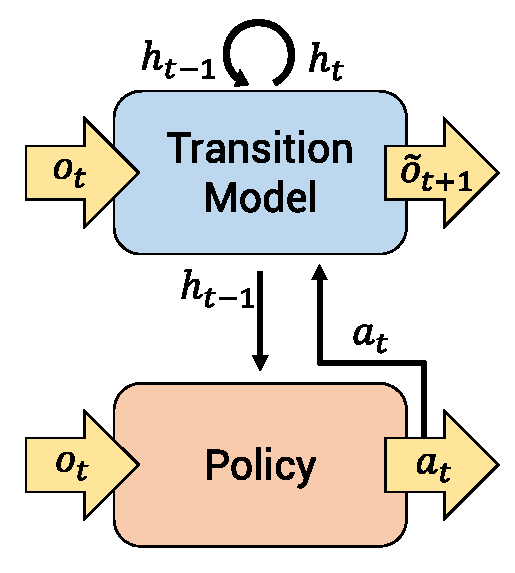
\includegraphics[width=0.4\linewidth]{imagenes/cap4/model_based_dcoach.png}
    \caption{Low-dimensional architecture for POMDP problems.}
    \label{fig:mb_dcoach}
\end{figure}

As Figure \ref{fig:mb_dcoach} shows, for training the model we assume that $(o_{t}, h_{t-1}) = s_{t}$ so that $M(o_{t}, h_{t-1},a_{t}) =M(s_{t},a_{t}) = s_{t+1}$ and $\pi(o_{t}, h_{t-1})=\pi(s_{t})=a_{t}$. Where $h_{t}$ is the hidden state of the LSTM layers computed at time step $t$.

\subsection{Low-dimensional State with Memory}
As it has been done previously in this work, we first study the low-dimensional state case. The objective is to learn the dynamics of the environment online i.e. as the policy is shaped interactively. 

If we look back to the approach taken in Chapter 2, the idea was similar. In that case the objective was to learn a low-dimensional embedding of a high-dimensional input online. The strategy was to share the encoder layers of an autoencoder between the policy and the autoencoder and update them using both the cost of the policy and the one of the autoencoder. In this case, the hidden state of the LSTM could be interpreted as an embedding of past observations. So, this recurrent layers could be shared between the policy and the model, updating them using both costs. A simplified version of this approach is shown in Figure \ref{fig:ld_model_rip}.

\begin{figure}[h]
    \centering
    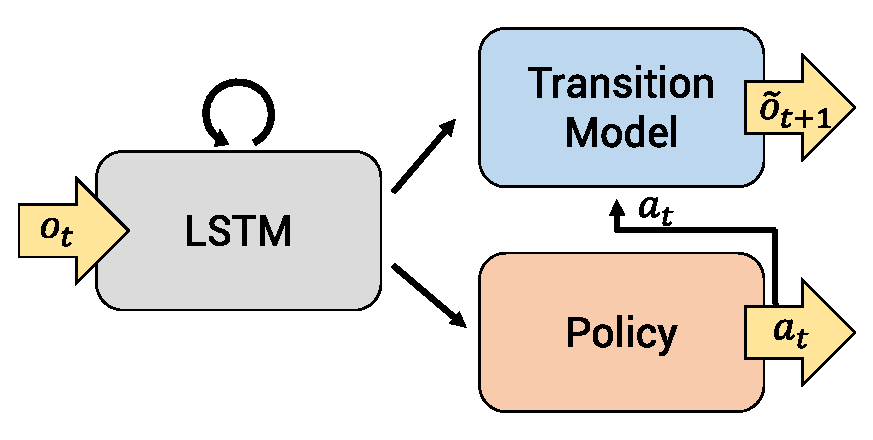
\includegraphics[width=0.6\linewidth]{imagenes/cap4/ld_model_rip.png}
    \caption{Low-dimensional architecture for POMDP problems.}
    \label{fig:ld_model_rip}
\end{figure}

The shortcoming presented in the approach shown in Figure \ref{fig:ld_model_rip} is that in this case the same problem that we found in the preliminary tests appears. The error of the policy does not work well when updating the weights of recurrent layers using the D-COACH strategy, even when using the auxiliary cost of the model. 

Alternatively, the approach was finally used is to update the model and the policy separately. If we go back to Figure \ref{fig:mb_dcoach}, this would mean that the \textbf{Model} box is updated with transitions collected by the agent, and, separately, the \textbf{Policy} box is updated with corrective feedback. The proposed model architecture consists of LSTM and FNN layers, as shown in Figure \ref{fig:ld_model_win}.

\begin{figure}[h]
    \centering
    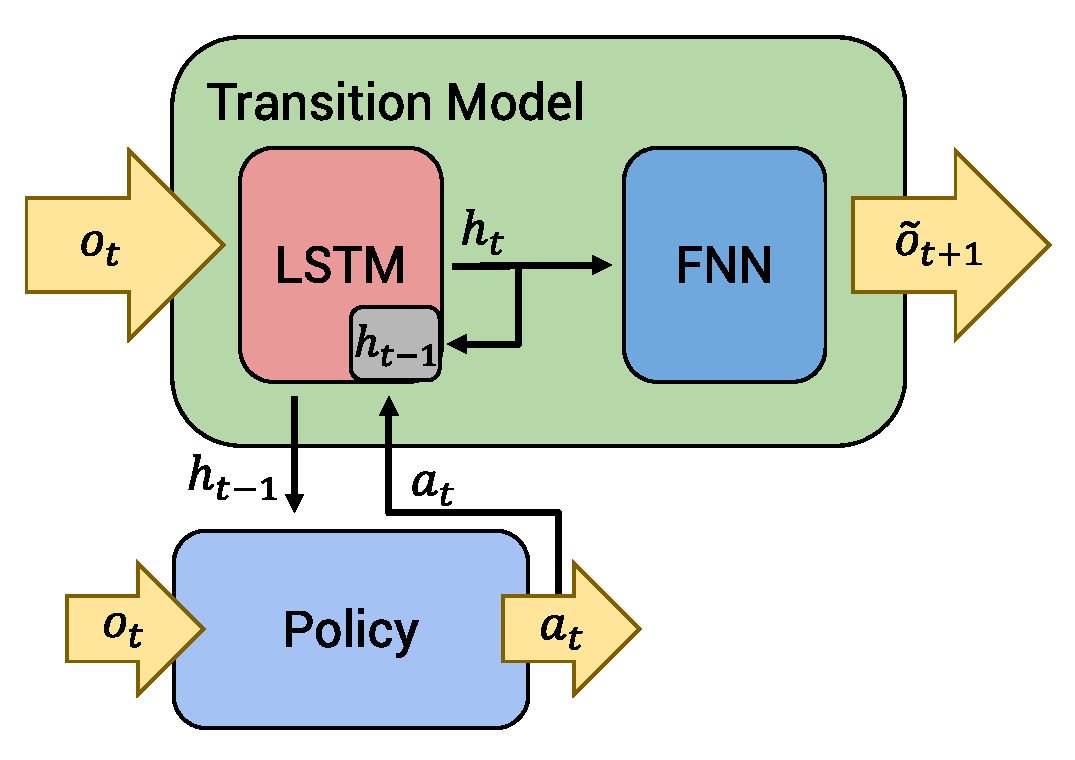
\includegraphics[width=0.7\linewidth]{imagenes/cap4/ld_model.png}
    \caption{Low-dimensional architecture for POMDP problems.}
    \label{fig:ld_model_win}
\end{figure}

The policy architecture is simply a compositions of FNN layers, as it is done in the other variations of D-COACH.

\subsection{High-dimensional State with Memory}
In the high-dimensional case, agents need to learn two embeddings: (1) spatial and (2) temporal. By spatial we mean a low-dimensional representation of high-dimensional data, which is what has been covered in the past chapters using autoencoders. By temporal we mean encapsulating previous observations in a memory, which is what has been done in the previous section using LSTMs. 

In preliminary tests, we found that the most effective way of doing this under the setting of D-COACH is to treat the autoencoder and the recurrent layers as one architecture, which represents the model. A model with the capability of learning from high-dimensional states, as it can be seen in Figure \ref{fig:rnn_hd}. 

\begin{figure}[h]
    \centering
    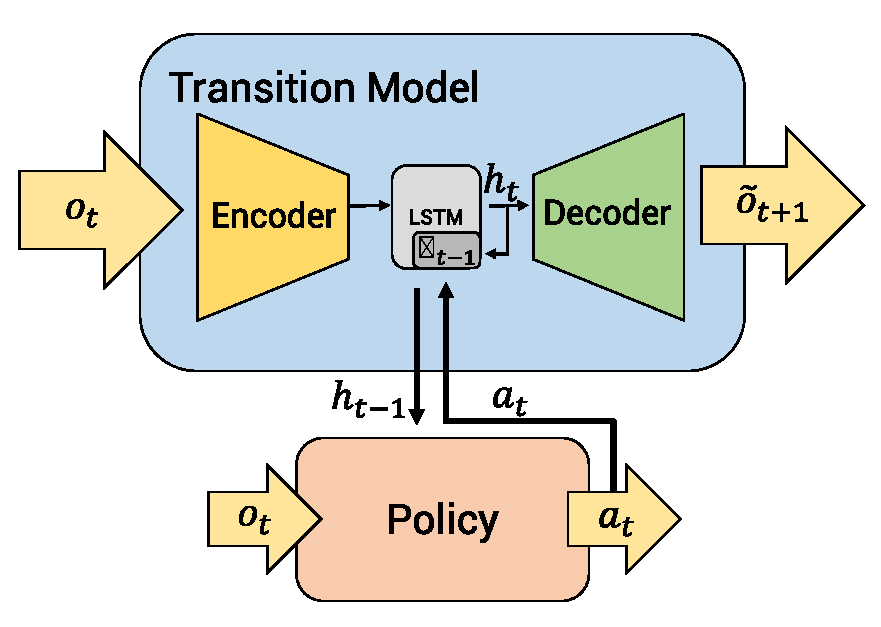
\includegraphics[width=0.8\linewidth]{imagenes/cap4/hd_model.png}
    \caption{High-dimensional architecture for POMDP problems.}
    \label{fig:rnn_hd}
\end{figure}

Instead of using a cost for the model and one for the autoencoder, we use the autoencoding cost but for reconstructing $s_{t+1}$. So, Equation \ref{eq:ae} instead of being $L(x_{t},\widetilde x_{t})$ it would be  $L(x_{t},\widetilde x_{t+1})$. By doing this, the hidden state of the LSTM embeds both the high-dimensional input and past observations.
\newpage

\subsection{The Algorithm}

In Algorithm \ref{algorithm:DeepCOACH-M}, the pseudocode of model-based D-COACH is presented. The hidden state of the LSTM is denoted as  $h^{\mathrm{LSTM}}$ and the human corrective feedback as  $h$.

\begin{algorithm}[h]
\caption{Model-based D-COACH for POMDPs}\label{algorithm:DeepCOACH-M}
\begin{algorithmic}[1]
\State \textbf{Require:} error magnitude $e$, policy buffer update interval $b$, policy buffer sampling size $N$, policy buffer min. size $k$, policy buffer max. size $K$, model buffer update interval $d$, model buffer sampling size $M$, model buffer min. size $l$, model buffer max. size $L$, training sequence length $\tau$.
\State \textbf{Init:} $\mathcal{B} = []$  \emph{\# initialize policy memory buffer}
\State \textbf{Init:} $\mathcal{D} = []$  \emph{\# initialize model memory buffer}
\For{t = 1,2,...}{}
\State \textbf{observe} observation $o_{t}$
\State \textbf{execute} action $a_{t}=\pi(o_{t}, h^{\mathrm{LSTM}}_{t-1})$
\State \textbf{feedback} human corrective advice $h_{t}$
\State \textbf{compute} $h^{\mathrm{LSTM}}_{t}$ from $M(o_{t}, a_{t},h^{\mathrm{LSTM}}_{t-1})$
\State \textbf{append} $(o_{t-1},...,o_{t-\tau},a_{t-1},...,a_{t-\tau},o_{t})$ to $\mathcal{D}$
\If{length($\mathcal{D}$) $> L$ }
\State $\mathcal{D} = \mathcal{D}[2:L+1]$
\EndIf
\If{$h_{t}$ is not \textbf{0}}
\State $\mathit{error}_{t} = h_{t}\cdot e$
\State $y_{label(t)} = a_{t} + \mathit{error}_{t}$ 
\State \textbf{update} $\pi$ using SGD with $(o_{t}, h^{\mathrm{LSTM}}_{t-1}, y_{\mathit{label}(t)})$ 
\State \textbf{update} $M$ using SGD with a mini-batch of sequences sampled from $\mathcal{D}$
\State \textbf{update} $\pi$ using SGD with a mini-batch of sequences sampled from $\mathcal{B}$
\State \textbf{append} $(o_{t},...,o_{t-\tau},a_{t-1},...,a_{t-\tau}, y_{\mathit{label}(t)})$ to $\mathcal{B}$
\If{length($\mathcal{B}$) $> K$ }
\State $\mathcal{B} = \mathcal{B}[2:K+1]$
\EndIf
\EndIf
\If{mod(t, b) is 0 and length($\mathcal{B}$) $\geq$ $k$}
\State \textbf{update} $\pi$ using SGD with a mini-batch of sequences sampled from $\mathcal{B}$
\EndIf
\If{mod(t, d) is 0 and length($\mathcal{D}$) $\geq$ $l$}
\State \textbf{update} $M$ using SGD with a mini-batch of sequences sampled from $\mathcal{D}$
\EndIf
\EndFor
\end{algorithmic}
\end{algorithm}


\section{Experiments and Results}
Simulated teachers were used in three different problems for validating model-based D-COACH. The main idea behind these experiments is to compare model-based D-COACH with model-free D-COACH (the one presented in Chapter 2) in partially observed problems.

\begin{enumerate}
    \item \textbf{Partially Observed Cart-Pole:} A partially observed low-dimensional state scenario. This is the same environment used in Chapter 1 with a modification in the observation space of the agent. In the standard fully-observable cart-pole the state has four dimensions, which consists of the position $x$ and velocity $\dot x$ of the cart and the angle $\theta$ and angular velocity $\dot \theta$ of the pole, such that $s=[x, \dot x, \theta, \dot \theta]$. In this case, we take out the derivatives present in the state, such that $s=[x, \theta]$.
    \item \textbf{Partially Observed Cart-Pole from Pixels:} The cart-pole environment is modified to use as input raw pixels (high-dimensional state). 
    \item \textbf{Partially Observed Car Racing:} A partially observed high-dimensional state scenario. The Car Racing problem presented in Chapter 1 is modified such that the indicators in the bottom of the image are gone. 
    
\end{enumerate}

\subsection{Validation Low-Dimensional State}

Model-based D-COACH is tested in the partially observed cart-pole because is a way to validate if the proposed methodology works in a simple setting. Figure \ref{fig:ld_cartpole_model} shows the learning curves of D-COACH with and without model. 

\begin{figure}[h]
    \centering
    \includegraphics[width=0.9\linewidth]{imagenes/cap3/cartpole_LD_model.pdf}
    \caption{Evolution of the error while learning the reacher task. }
    \label{fig:ld_cartpole_model}
\end{figure}

Model-free D-COACH is not able to learn a well performing policy in this case. This was something to expect given that the velocities of both the cart and the pole are essential for making good decisions in a problem of these characteristics. Figure \ref{fig:cp_ex} shows and example of two scenarios in where at time step 2 the observation would be the same in the partially observed cart-pole (if we only focus on the angle of the pole). In this example the angular velocity of the pole changes direction between scenarios, but an agent without memory is not able to tell the difference. As a consequence, in $t=2$, it would make the same decision in two opposite scenarios.

\begin{figure}[h]
    \centering
    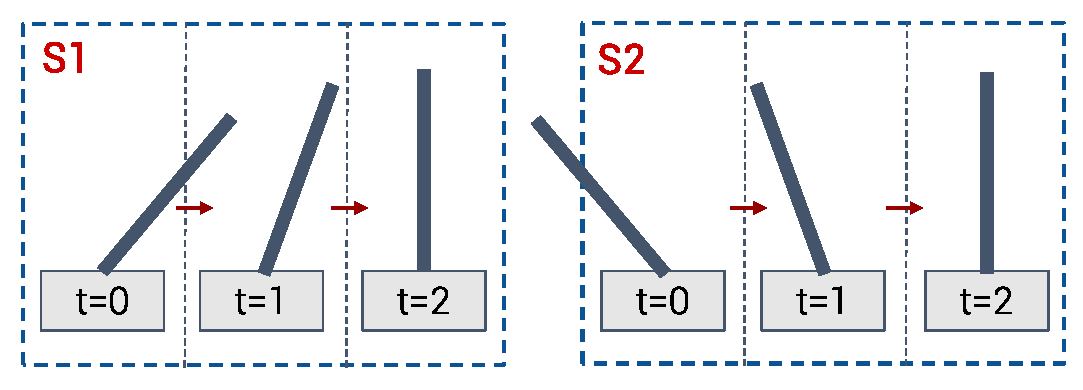
\includegraphics[width=0.9\linewidth]{imagenes/cap4/cartpole_ex.png}
    \caption{Evolution of the error while learning the reacher task. }
    \label{fig:cp_ex}
\end{figure}

In contrast, if the agent makes decisions based on previous observations it can understand that these two scenarios are different and take better decisions. This is shown in the blue curve of Figure \ref{fig:cp_ex}, where the agent is able to learn a well performing policy in about 12 minutes. 

\subsection{Validation High-Dimensional State}
In this section we validate model-based D-COACH in two different problems. Cart-pole is a problem that was not originally designed to be solved using as input raw pixels of an image, so we do not expect to obtain a perfect performance. The main goal of testing D-COACH with this problem is to observe if the proposed model (autoencoder + LSTM) is able to embed both the past and high-dimensional inputs adequately.

\begin{figure}[h]
    \centering
    \includegraphics[width=0.9\linewidth]{imagenes/cap3/cartpole_HD_model.pdf}
    \caption{Evolution of the error while learning the reacher task. }
    \label{fig:cp_hd}
\end{figure}

Figure \ref{fig:cp_hd} shows a much more slower learning speed if we compare these agents with the ones of Figure \ref{fig:cp_ex}. This is something to expect given that now the agents are also learning to extract features from the image. Also, model-free D-COACH shows a faster learning speed at the beginning, but after 8 minutes of learning it is outperformed by model-based D-COACH. This shows that D-COACH takes longer to learn a temporal/spatial embedding than just a spatial embedding. But, in POMDPs, eventually, model-based D-COACH should outperform its model-free version.

Finally, model-based D-COACH was validated in the partially observed Car Racing problem. Figure \ref{fig:po_cr} shows that model-free D-COACH is able to learn a well-performing policy even though the state is partially observed. Nevertheless, model-based D-COACH shows that it is possible to obtain an even better performance if memory is added to the policy. The difference between both curves shows that model-based D-COACH is a more robust and powerful approach than model-free D-COACH, capable of enhancing the performance of the agent in problems where model-free D-COACH could appear to be sufficient.

\begin{figure}[h]
    \centering
    \includegraphics[width=0.9\linewidth]{imagenes/cap3/car_racing_lstm.pdf}
    \caption{Evolution of the error while learning the reacher task. }
    \label{fig:po_cr}
\end{figure}

\section{Discussion}
In this chapter we introduced a variation of D-COACH with memory, model-based D-COACH. The main objective was to extend D-COACH in order for it to work in the set of POMDPs where the state is described by time-dependent phenomena. Low-dimensional and high-dimensional problems were covered, introducing a different model architecture for each case. 

Model-based D-COACH offers a framework that learns both the policy and the model online. This makes it easy for humans to interact in the learning process of the agents, given that no human effort is needed in extra learning steps as in the offline state learning version of D-COACH (Chapter 2). The experiments show that the proposed method is effective for enhancing the performance of agents in POMDPs. As discussed previously, memory-based approaches may be key to solve problems in real-world scenarios, where is common to face problems with partial observability. 

As it is stated in the overview of this chapter, RNNs have an extra overhead when training, because sequences must be used for updating the weights of the recurrent layers. Given that D-COACH is an IML approach, updates are done in real-time while the teacher is providing feedback. We found that the overhead produced when updating the recurrent layers is too high for running this approach in CPU; thus, a GPU was used. This is a disadvantage with respect to the previously proposed variations of D-COACH, given that those models are able to run in real-time using CPUs. 